\section{Benchmark Implementation}
\label{sec: benchmark-implementation}
This chapter presents the implementation details of our benchmarking framework, designed to evaluate the performance of geo-distributed transactional systems based on the PPS workloads. We discuss here key design choices, such as the integration of the benchmarking framework with the evaluated databases (Section~\ref{subsec: integration-with-different-databases}), the support for dependent transactions (Section~\ref{subsec: dependent-transactions}), the custom partitioning and home assignment schemes that offer precise control over transaction configurations (Section~\ref{subsec: partitioning-and-home-assignment-schemes}), and the transactional mix of the workload (Section~\ref{subsec: transactional-mix}).

\begin{figure}[ht]
    \centering
    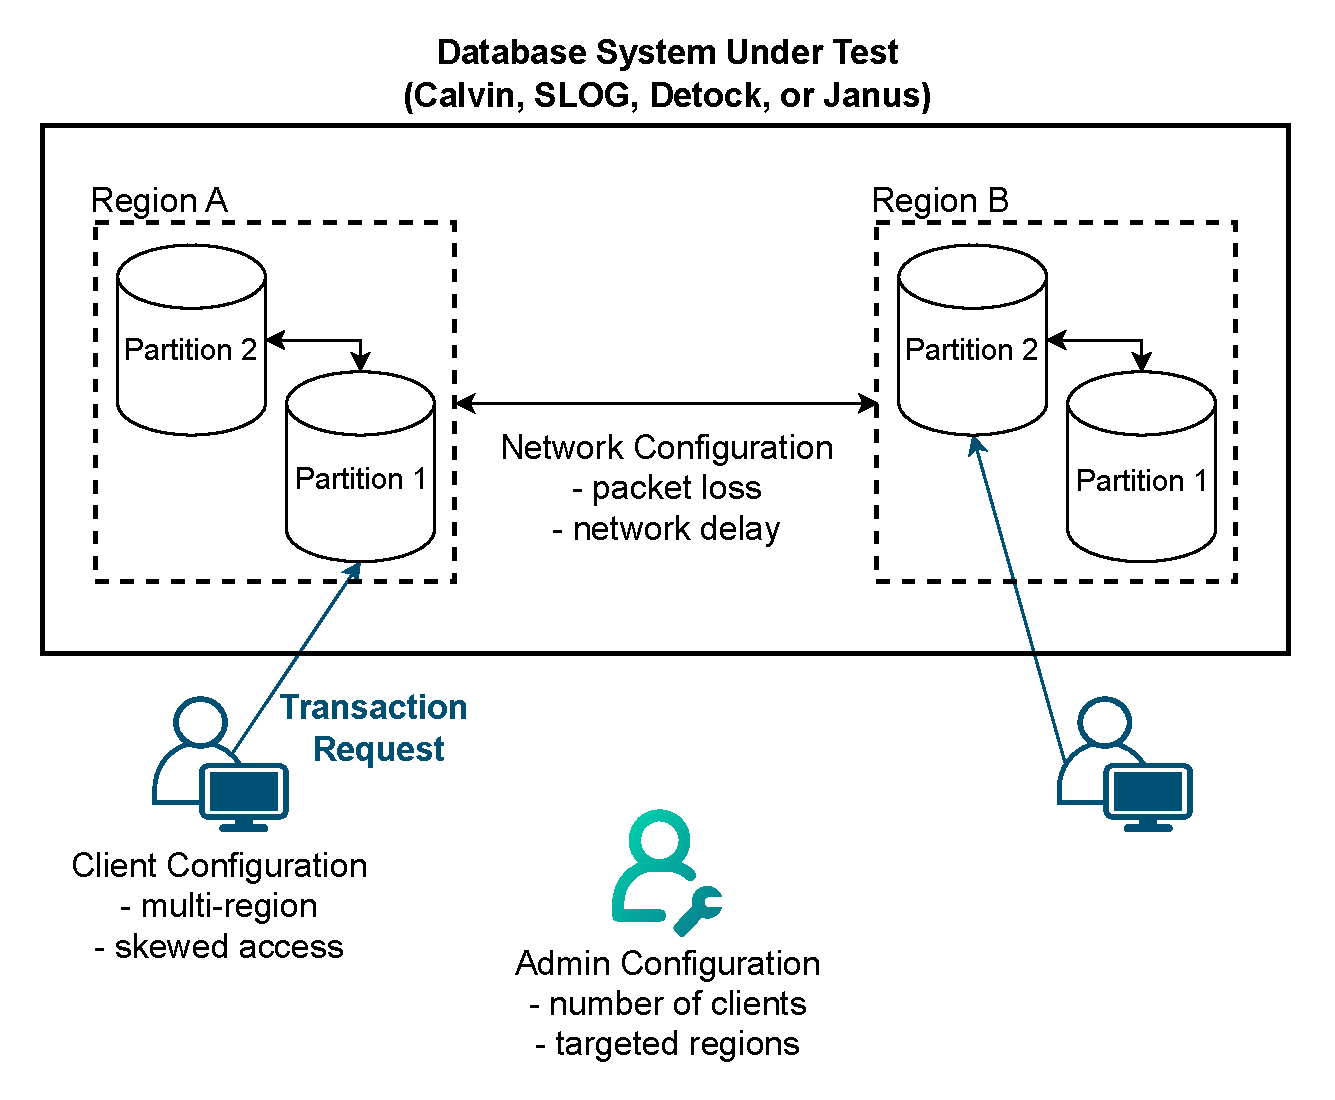
\includegraphics[width=1\linewidth]{figures/Overall Architecture.pdf}
    \caption{Overall Architecture of the Benchmarking Framework, along with all the Tunable Parameters}
    \label{fig: overall-architecture}
\end{figure}

\subsection{Integration with Different Databases}
\label{subsec: integration-with-different-databases}
The databases we evaluate follow a common setup, where data is partitioned across different servers, and each partition is replicated in several different geographically distributed regions to ensure availability and low latency by placing the data closer to the users. Our benchmark is capable of spawning clients in different regions and targeting specific partitions within that region. The overall architecture of our benchmarking framework and the way it interacts with geo-distributed databases is shown in Figure~\ref{fig: overall-architecture}.

As stated in Section~\ref{subsec: evaluated-systems}, we implemented the benchmark within the Detock codebase to offer a unified testing environment for all the evaluated systems. This integration also allows us to define key components such as table schemas, table loaders, and stored procedures in a single place and use them consistently across all databases.

\subsection{Dependent Transactions}
\label{subsec: dependent-transactions}
We mentioned in Section~\ref{subsec: evaluated-systems} that all the evaluated databases need to know the complete set of accessed records for each transaction to either deterministically order them or construct the serialization graph. Among the transactions specific to the PPS workload, only \textit{OrderProduct} is a dependent transaction since it must first determine which parts are associated with the product before any updates can take place. 

In its original design, Calvin was implemented to support dependent transactions by using a scheme called Optimistic Lock Location Prediction (OLLP) that makes use of a reconnaissance query to perform all the necessary reads to compute the complete read/write set before the actual execution begins. Unfortunately, this mechanism is not currently implemented in the Detock framework. As a solution, we'll use a similar approach by splitting the \textit{OrderProduct} transaction into \textit{two client-side phases}. In the first phase, the client fetches the current list of parts associated with the given product. Then, in the second phase, the client issues the update request with the complete set of accessed records. It's important to note that when the second phase detects any changes in the reads done by the first phase, it will self-abort.

\subsection{Partitioning and Home Assignment Schemes.}
\label{subsec: partitioning-and-home-assignment-schemes}
Our benchmark supports custom partitioning schemes. In our setup, we partitioned the data across nodes in a round-robin fashion based on the record identifier (\texttt{product\_id}, \texttt{part\_id}, \texttt{supplier\_id}) for the core entities and the \texttt{product\_id} for the two additional relationship tables. We say that a transaction is \textit{single-partition} if it accesses data from only one partition, and \textit{multi-partition} if it spans multiple partitions.

In addition to partitioning, SLOG and Detock use a couple of optimizations based on the concept of \textit{home regions}. In short, each record is assigned to exactly one geographical region, which is called the home region of this record and is responsible for coordinating the access to that record. Both systems assume that, theoretically, within each region, data is partitioned locally regardless of which region owns the data. This means that a single partition can hold records whose home regions are different. Similar to partitioning, we can classify the transactions into \textit{single-home} and \textit{multi-home}. Our implementation supports custom home assignment schemes. In our evaluation, we assign home regions in a round-robin fashion within each partition for simplicity.

In our workload, only the second phase of the \textit{OrderProduct} transaction can be configured to be either single-partition or multi-partition, and independently, single-home or multi-home, depending on which parts are involved. The other transactions are simpler, since they either access only one record or all the accessed records fall within a single partition and home region, according to the chosen partitioning and home assignment scheme. The main challenge in configuring the second phase of the \textit{OrderProduct} transaction is that we don't know which parts will be accessed in advance. To overcome this, when creating the tables, we split the products into four groups based on the distribution of their parts:
\begin{itemize}
    \item \textit{Category I}. All parts are located in the same partition and have the same home region as the product itself.
    \item \textit{Category II}. All parts are located in the same partition as the product, but belong to different home regions.
    \item \textit{Category III}. All parts have the same home region as the product, but are located in different partitions.
    \item \textit{Category IV}. The parts are located in different partitions and also belong to different home regions.
\end{itemize}

\subsection{Transactional Mix}
\label{subsec: transactional-mix}
Section~\ref{subsec: product-parts-supplier-workload} introduced the type of transactions that we consider in our benchmarking framework. While all these transactions reflect realistic business operations, such as updating a product or retrieving a part, not all of these types are well-suited for evaluating geo-distributed behavior. In particular, as stated in the previous subsection, only the \textit{OrderProduct} transaction has an access pattern that can span multiple partitions and regions, making it the only meaningful operation that can test the servers' coordination.

As a consequence, we used a transactional mix that favored using the \textit{OrderProduct} type. In addition, we assigned greater weights to the \textit{UpdateProductPart} type since it can interfere with the two-phase dependent transactions, and to the \textit{GetPartsByProduct} type since it accesses multiple records, which makes it more relevant for evaluating concurrency behavior. In contrast, the simple read-only transactions \textit{GetPart} and \textit{GetProduct} have lower priority. Therefore, our experiments use a transactional mix consisting of 70\% \textit{OrderProduct}, 10\% \textit{GetPartsByProduct}, 10\% \textit{UpdateProductPart}, 5\% \textit{GetProduct}, and 5\% \textit{GetPart}.